\documentclass{beamer}\usepackage[]{graphicx}\usepackage[]{color}
% maxwidth is the original width if it is less than linewidth
% otherwise use linewidth (to make sure the graphics do not exceed the margin)
\makeatletter
\def\maxwidth{ %
  \ifdim\Gin@nat@width>\linewidth
    \linewidth
  \else
    \Gin@nat@width
  \fi
}
\makeatother

\definecolor{fgcolor}{rgb}{0.345, 0.345, 0.345}
\newcommand{\hlnum}[1]{\textcolor[rgb]{0.686,0.059,0.569}{#1}}%
\newcommand{\hlstr}[1]{\textcolor[rgb]{0.192,0.494,0.8}{#1}}%
\newcommand{\hlcom}[1]{\textcolor[rgb]{0.678,0.584,0.686}{\textit{#1}}}%
\newcommand{\hlopt}[1]{\textcolor[rgb]{0,0,0}{#1}}%
\newcommand{\hlstd}[1]{\textcolor[rgb]{0.345,0.345,0.345}{#1}}%
\newcommand{\hlkwa}[1]{\textcolor[rgb]{0.161,0.373,0.58}{\textbf{#1}}}%
\newcommand{\hlkwb}[1]{\textcolor[rgb]{0.69,0.353,0.396}{#1}}%
\newcommand{\hlkwc}[1]{\textcolor[rgb]{0.333,0.667,0.333}{#1}}%
\newcommand{\hlkwd}[1]{\textcolor[rgb]{0.737,0.353,0.396}{\textbf{#1}}}%
\let\hlipl\hlkwb

\usepackage{framed}
\makeatletter
\newenvironment{kframe}{%
 \def\at@end@of@kframe{}%
 \ifinner\ifhmode%
  \def\at@end@of@kframe{\end{minipage}}%
  \begin{minipage}{\columnwidth}%
 \fi\fi%
 \def\FrameCommand##1{\hskip\@totalleftmargin \hskip-\fboxsep
 \colorbox{shadecolor}{##1}\hskip-\fboxsep
     % There is no \\@totalrightmargin, so:
     \hskip-\linewidth \hskip-\@totalleftmargin \hskip\columnwidth}%
 \MakeFramed {\advance\hsize-\width
   \@totalleftmargin\z@ \linewidth\hsize
   \@setminipage}}%
 {\par\unskip\endMakeFramed%
 \at@end@of@kframe}
\makeatother

\definecolor{shadecolor}{rgb}{.97, .97, .97}
\definecolor{messagecolor}{rgb}{0, 0, 0}
\definecolor{warningcolor}{rgb}{1, 0, 1}
\definecolor{errorcolor}{rgb}{1, 0, 0}
\newenvironment{knitrout}{}{} % an empty environment to be redefined in TeX

\usepackage{alltt}
\IfFileExists{upquote.sty}{\usepackage{upquote}}{}
\begin{document}

\begin{frame} 
\frametitle{Exercício 1: Praticando Latex} 
Texto, conteúdo normal 
Mais texto 
\end{frame}



\begin{frame} 
\frametitle{Exercício 1: Praticando Latex} 

1) Usando o formato “.Rnw”, crie um PDF com texto simples usando pelo menos cinco das formatações acima.\hfill\break

Meu nome é \textbf{Beatriz Milz}, atualmente eu faço \texttt{doutorado} no \emph{PROCAM/IEE/USP}. \break


Coisas que gosto:

\begin{itemize}
  \item Fazer parte de comunidades
  \item Itens de papelaria
  \item Completar tarefas atrasadas
\end{itemize}


Coisas para comprar quando for ao mercado:

\begin{enumerate}
  \item Café
  \item Chocolate
\end{enumerate}

\end{frame}


\begin{frame} 
\frametitle{Exercício 1: Praticando Latex} 
2) Adicione a famosa equação de Pythagoras.

$$a^{2} = b^{2} + c^{2} $$
\end{frame}





3) Adicione uma tabela simples usando o banco de dados de weather que mostra o total de precipitação por mês:

\begin{knitrout}
\definecolor{shadecolor}{rgb}{0.969, 0.969, 0.969}\color{fgcolor}\begin{kframe}
\begin{alltt}
\hlkwd{library}\hlstd{(nycflights13)}
\hlkwd{library}\hlstd{(tidyverse)}

\hlstd{nycflights13}\hlopt{::}\hlstd{weather} \hlopt
  \hlkwd{group_by}\hlstd{(month)} \hlopt
  \hlkwd{summarise}\hlstd{(}\hlkwc{total_precip} \hlstd{=} \hlkwd{sum}\hlstd{(precip,} \hlkwc{na.rm} \hlstd{=} \hlnum{FALSE}\hlstd{))} \hlopt
  \hlstd{knitr}\hlopt{::}\hlkwd{kable}\hlstd{(}\hlkwc{format} \hlstd{=} \hlstr{"latex"}\hlstd{,}
               \hlkwc{col.names} \hlstd{=} \hlkwd{c}\hlstd{(}\hlstr{"Mês"}\hlstd{,} \hlstr{"Precipitação acumulada"}\hlstd{),}
               \hlkwc{align} \hlstd{=} \hlstr{"c"}\hlstd{,}
               \hlkwc{caption} \hlstd{=} \hlstr{"Precipitação acumulada por mês (inches)"}
               \hlstd{)}
\end{alltt}
\end{kframe}\begin{table}

\caption{\label{tab:unnamed-chunk-1}Precipitação acumulada por mês (inches)}
\centering
\begin{tabular}[t]{c|c}
\hline
Mês & Precipitação acumulada\\
\hline
1 & 8.50\\
\hline
2 & 9.72\\
\hline
3 & 7.66\\
\hline
4 & 4.40\\
\hline
5 & 13.71\\
\hline
6 & 24.84\\
\hline
7 & 8.80\\
\hline
8 & 9.27\\
\hline
9 & 6.75\\
\hline
10 & 1.25\\
\hline
11 & 8.30\\
\hline
12 & 13.51\\
\hline
\end{tabular}
\end{table}


\end{knitrout}



4) Adicione um gráfico simples usando o banco de dados weather que mostra a temperatura média por aeroporto.
Verifique que o seu documento compila bem para PDF.

\begin{knitrout}
\definecolor{shadecolor}{rgb}{0.969, 0.969, 0.969}\color{fgcolor}\begin{kframe}
\begin{alltt}
\hlstd{nycflights13}\hlopt{::}\hlstd{weather} \hlopt
  \hlkwd{group_by}\hlstd{(origin)} \hlopt
  \hlkwd{summarise}\hlstd{(}\hlkwc{t_media} \hlstd{=} \hlkwd{mean}\hlstd{(temp,} \hlkwc{na.rm} \hlstd{=} \hlnum{TRUE}\hlstd{))} \hlopt
  \hlkwd{ggplot}\hlstd{()} \hlopt{+}
  \hlkwd{geom_col}\hlstd{(}\hlkwd{aes}\hlstd{(}\hlkwc{x} \hlstd{= origin,} \hlkwc{y} \hlstd{= t_media),} \hlkwc{fill} \hlstd{=} \hlstr{"lightblue"}\hlstd{)} \hlopt{+}
  \hlkwd{labs}\hlstd{(}
    \hlkwc{x} \hlstd{=} \hlstr{"Aeroporto"}\hlstd{,}
    \hlkwc{y} \hlstd{=} \hlstr{"Temperatura média (ºF)"}
  \hlstd{)}
\end{alltt}
\end{kframe}
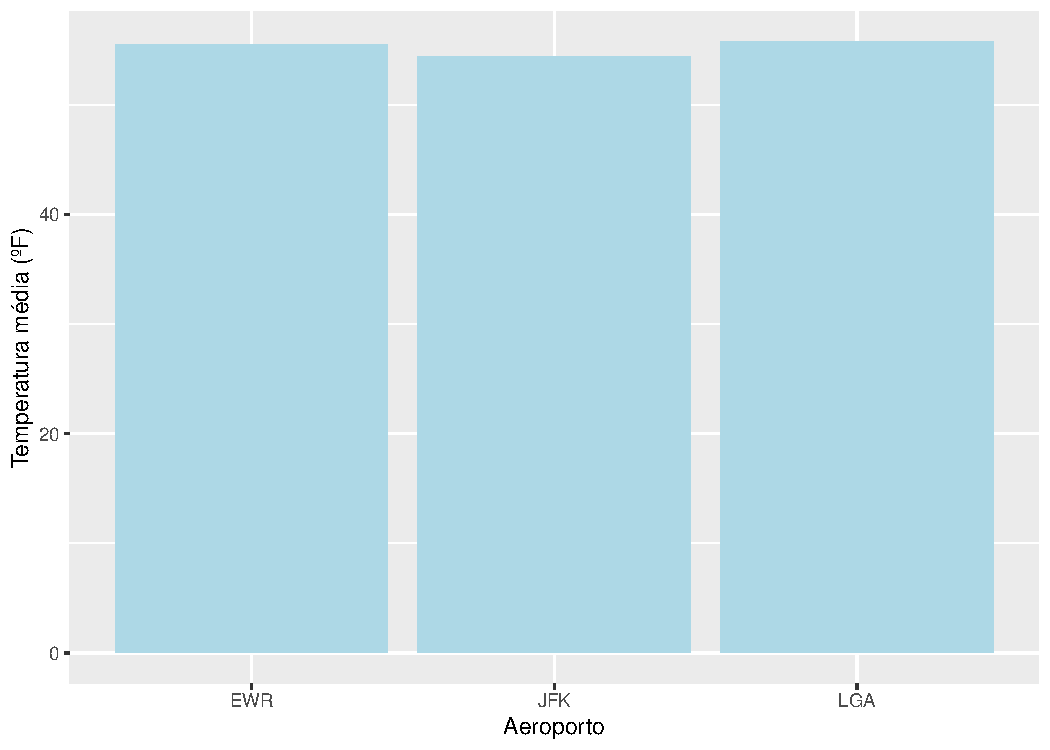
\includegraphics[width=\maxwidth]{figure/unnamed-chunk-2-1} 

\end{knitrout}



5) Ajuste o seu script “.Rnw” acima para gerar uma apresentão do class ‘beamer’ e coloca o texto, a equação, a tabela, e o gráfico em slides diferentes. Compile para PDF de novo.

\textbf{Resposta em outro arquivo. }

\end{document}
